\chapter{Execução do Estudo de Caso e Análise dos Dados}
\label{chap:execucao}

Neste capítulo serão apresentadas as análises dos dados quantitativos e qualitativos e a discussão dos resultados.


\section{Analises do SIGET}

Para cada uma das \textit{releases} do SIGET, coletou-se o código-fonte, conforme a disponibilidade, no repositório da CAIXA. Após a obtenção do código-fonte,foi realizado a análise estática cada \textit{release} utilizando as ferramentas analizo, findbugs e PMD. Posteriormente, os resultados das análises foram extraídos, transformados e carregados no ambiente de Data Warehousing proposto no Capítulo \ref{chap:arquitetura}. Dessa forma, foi possível obter:

\begin{easylist}[itemize]

& O intervalo qualitativo para cada uma das Métricas de Código-Fonte por \textit{index} e por \textit{release}; 

& Quantidade de Cenários de Limpeza total, por tipo e por \textit{release}; 

& Classe, nome e recomendação para cada cenário de limpeza; 

& Quantidade de \textit{bugs} total,por tipo, por \textit{index} e por \textit{release};

& Classe, tipo, nome e linha para cada \textit{bug}; 

& Quantidade de violações total,por tipo, por \textit{index} e por \textit{release};

& Classe, tipo, nome e linha para cada violação; 

\end{easylist}

Como demonstrado nas Figuras \ref{dashboardtotal}, \ref{dashboardPMD}, \ref{dashboardFindbugs} e \ref{dashboardCenarios}.

\begin{figure}[h!]
\centering
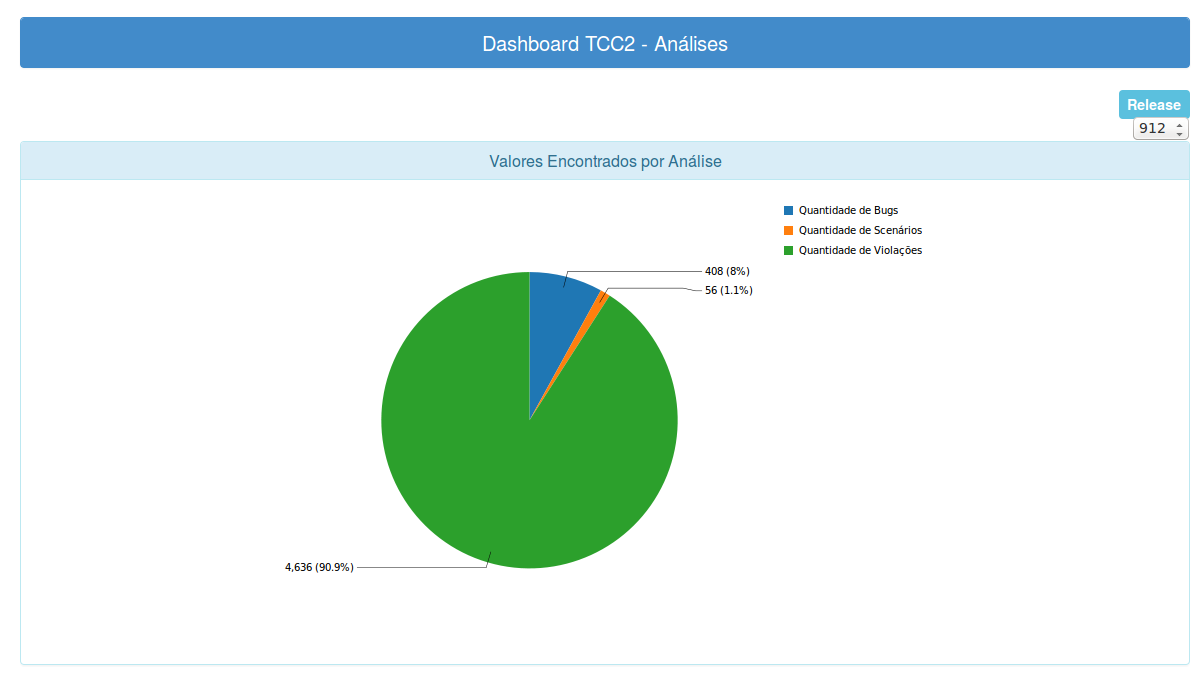
\includegraphics[keepaspectratio=false,scale=0.4]{figuras/figuras_nilton/DashboardTotal.eps}
\caption{\textit{Dashboard} Quantidade Total}
\label{dashboardtotal}
\end{figure}

\begin{figure}[h!]
\centering
\includegraphics[keepaspectratio=false,scale=0.5]{figuras/figuras_nilton/DashboardPMD.eps}
\caption{\textit{Dashboard PMD}}
\label{dashboardPMD}
\end{figure}

\begin{figure}[h!]
\centering
\includegraphics[keepaspectratio=false,scale=0.5]{figuras/figuras_nilton/DashboardCenarios.eps}
\caption{\textit{Dashboard} Cenários}
\label{dashboardFindbugs}
\end{figure}

\begin{figure}[h!]
\centering
\includegraphics[keepaspectratio=false,scale=0.5]{figuras/figuras_nilton/DashboardFindbugs.eps}
\caption{\textit{Dashboard FindBugs}}
\label{dashboardCenarios}
\end{figure}

\section{Analise do Questionário}

\section{Analise do Erro Quadrático Médio}

\section{Analise do Coeficiente de Correlação}
